% Source reference: :contentReference[oaicite:0]{index=0}
\part{Graph Theory}
\section{Handout 08: Graph Theory (2): Traversing Graphs}

\subsection{Overview}

This handout studies how to traverse graphs. The main objects are paths, circuits, connectivity, Euler paths/circuits, and Hamilton paths/circuits.

The central distinction is:
\[
\text{Euler: use every edge exactly once}
\qquad\text{versus}\qquad
\text{Hamilton: visit every vertex exactly once}.
\]

The main topics are:
\begin{itemize}[leftmargin=*]
    \item directed graphs and in-degree/out-degree;
    \item directed Handshaking Lemma;
    \item paths, simple paths, circuits, and length;
    \item connected components in undirected graphs;
    \item strongly and weakly connected directed graphs;
    \item Euler circuits and Euler paths;
    \item Hamilton circuits and Hamilton paths.
\end{itemize}

\begin{examtip}[title={Main diagnostic for Handout 08}]
Before solving a traversing-graph problem, decide whether the condition is about:
\[
\text{reachability},\qquad
\text{using edges},\qquad
\text{visiting vertices}.
\]
Connectivity is about reachability, Euler theory is about edges, and Hamilton theory is about vertices.
\end{examtip}

%==================================================
\subsection{Directed Graphs and Directed Degree}
%==================================================

\begin{definition}{Directed graph}{directed-graph-recall}
A graph \(G=(V,E)\) is \emph{directed} if every edge in \(E\) is an ordered pair of vertices. An edge
\[
e=(u,v)
\]
has direction from \(u\) to \(v\). The vertex \(u\) is the \emph{initial vertex} of \(e\), and \(v\) is the \emph{terminal vertex} of \(e\).
\end{definition}

\begin{definition}{In-degree and out-degree}{directed-degree}
Let \(G=(V,E)\) be a directed graph.
\begin{itemize}[leftmargin=*]
    \item The \emph{in-degree} of a vertex \(v\), denoted \(\deg^{-}(v)\), is the number of directed edges whose terminal vertex is \(v\).
    \item The \emph{out-degree} of a vertex \(v\), denoted \(\deg^{+}(v)\), is the number of directed edges whose initial vertex is \(v\).
\end{itemize}
A self-loop at \(v\) contributes \(1\) to \(\deg^{-}(v)\) and \(1\) to \(\deg^{+}(v)\).
\end{definition}

% Directed graph illustrating in-degrees and out-degrees.
\begin{center}
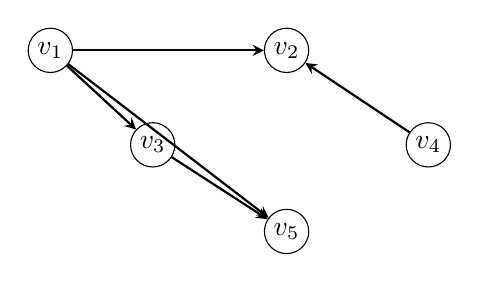
\begin{tikzpicture}[>=stealth,scale=1.0]
    \node[circle,draw,inner sep=1.8pt] (v1) at (0,1.2) {$v_1$};
    \node[circle,draw,inner sep=1.8pt] (v2) at (3,1.2) {$v_2$};
    \node[circle,draw,inner sep=1.8pt] (v3) at (1.3,0) {$v_3$};
    \node[circle,draw,inner sep=1.8pt] (v5) at (3.0,-1.1) {$v_5$};
    \node[circle,draw,inner sep=1.8pt] (v4) at (4.8,0) {$v_4$};

    \draw[->,thick] (v1) -- (v2);
    \draw[->,thick] (v1) -- (v3);
    \draw[->,thick] (v1) -- (v5);
    \draw[->,thick] (v4) -- (v2);
    \draw[->,thick] (v3) -- (v5);
\end{tikzpicture}
\end{center}

\begin{examplebox}[title={Directed degree calculation}]
For the directed graph with
\[
V=\{v_1,v_2,v_3,v_4,v_5\}
\]
and
\[
E=\{(v_1,v_2),(v_1,v_3),(v_1,v_5),(v_4,v_2),(v_3,v_5)\},
\]
the degrees are:
\[
\deg^{-}(v_1)=0,\quad \deg^{+}(v_1)=3,
\]
\[
\deg^{-}(v_2)=2,\quad \deg^{+}(v_2)=0,
\]
\[
\deg^{-}(v_3)=1,\quad \deg^{+}(v_3)=1,
\]
\[
\deg^{-}(v_4)=0,\quad \deg^{+}(v_4)=1,
\]
\[
\deg^{-}(v_5)=2,\quad \deg^{+}(v_5)=0.
\]
\end{examplebox}

\begin{theorem}{Directed Handshaking Lemma}{directed-handshaking}
Let \(G=(V,E)\) be a directed graph with \(m\) edges. Then
\[
\sum_{v\in V}\deg^{-}(v)
=
\sum_{v\in V}\deg^{+}(v)
=
m.
\]
\end{theorem}

\begin{proof}
Each directed edge has exactly one initial vertex and exactly one terminal vertex. Hence each edge contributes \(1\) to the total out-degree and \(1\) to the total in-degree. Summing over all \(m\) edges gives the result.
\end{proof}

\begin{keyformula}[title={Directed Handshaking Lemma}]
\[
\sum_{v\in V}\deg^{-}(v)=\sum_{v\in V}\deg^{+}(v)=|E|.
\]
\end{keyformula}

\begin{commonmistake}[title={Undirected degree versus directed degree}]
In an undirected graph, one edge contributes \(2\) to the total degree sum. In a directed graph, one directed edge contributes \(1\) to the total in-degree and \(1\) to the total out-degree separately.
\end{commonmistake}

%==================================================
\subsection{Paths, Simple Paths, and Circuits}
%==================================================

\begin{definition}{Path in an undirected graph}{undirected-path}
Let \(G=(V,E)\) be an undirected graph. A \emph{path} from \(u\) to \(v\) is a sequence of vertices
\[
(u=w_0,w_1,\dots,w_k,w_{k+1}=v)
\]
such that
\[
\{w_i,w_{i+1}\}\in E
\qquad
\text{for all }0\le i\le k.
\]
The \emph{length} of the path is the number of edges in the path.
\end{definition}

\begin{definition}{Path in a directed graph}{directed-path}
Let \(G=(V,E)\) be a directed graph. A \emph{directed path} from \(u\) to \(v\) is a sequence of vertices
\[
(u=w_0,w_1,\dots,w_k,w_{k+1}=v)
\]
such that
\[
(w_i,w_{i+1})\in E
\qquad
\text{for all }0\le i\le k.
\]
The direction of every edge must match the order in the vertex sequence.
\end{definition}

\begin{definition}{Simple path and circuit}{simple-path-circuit}
In this course, a \emph{simple path} is a path that contains no edge more than once.

If a path starts and ends at the same vertex, then it is called a \emph{circuit}.
\end{definition}

\begin{examtip}[title={Course convention for simple path}]
Some books define a simple path as one with no repeated vertices. In this course, the relevant definition is: \emph{no edge is repeated}. Use the course definition unless a question explicitly states otherwise.
\end{examtip}

% Graph for path and circuit examples.
\begin{center}
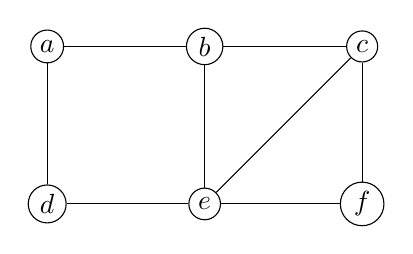
\begin{tikzpicture}[scale=1.0]
    \node[circle,draw,inner sep=1.8pt] (a) at (0,1) {$a$};
    \node[circle,draw,inner sep=1.8pt] (b) at (2,1) {$b$};
    \node[circle,draw,inner sep=1.8pt] (c) at (4,1) {$c$};
    \node[circle,draw,inner sep=1.8pt] (d) at (0,-1) {$d$};
    \node[circle,draw,inner sep=1.8pt] (e) at (2,-1) {$e$};
    \node[circle,draw,inner sep=1.8pt] (f) at (4,-1) {$f$};

    \draw (a)--(b)--(c)--(f)--(e)--(d)--(a);
    \draw (b)--(e);
    \draw (c)--(e);
\end{tikzpicture}
\end{center}

\begin{examplebox}[title={Reading paths from a graph}]
In the graph above:
\begin{itemize}[leftmargin=*]
    \item \(d-a-b-c-f\) is a simple path of length \(4\);
    \item \(d-e-c-b-a-d\) is a circuit of length \(5\);
    \item \(a-b,e-f\) is not a path, since there is no edge joining \(b\) to \(e\) in that sequence unless \(b-e\) is explicitly present;
    \item \(d-a-b-c-f-b-a-e\) would fail to be simple if an edge is reused.
\end{itemize}
\end{examplebox}

\begin{commonmistake}[title={A sequence of vertices is not automatically a path}]
A vertex sequence is a path only if every consecutive pair is joined by the required edge. In a directed graph, the edge direction must also agree with the order of the sequence.
\end{commonmistake}

%==================================================
\subsection{Connectivity}
%==================================================

\begin{definition}{Connected graph and components}{connected-components}
An undirected graph \(G=(V,E)\) is \emph{connected} if for every pair of vertices \(u,v\in V\), there is a path from \(u\) to \(v\).

If \(G\) is not connected, it is called \emph{disconnected}. Its maximal connected subgraphs are called its \emph{connected components}.
\end{definition}

% Connected versus disconnected graph.
\begin{center}
\begin{tikzpicture}[scale=1.0]
    \begin{scope}[shift={(0,0)}]
        \node at (1.8,1.7) {connected};
        \node[circle,draw,inner sep=1.5pt] (a) at (0,0) {};
        \node[circle,draw,inner sep=1.5pt] (b) at (1.2,1) {};
        \node[circle,draw,inner sep=1.5pt] (c) at (2.4,0) {};
        \node[circle,draw,inner sep=1.5pt] (d) at (1.2,-1) {};
        \draw (a)--(b)--(c)--(d)--(a);
        \draw (b)--(d);
    \end{scope}

    \begin{scope}[shift={(6,0)}]
        \node at (1.8,1.7) {disconnected};
        \node[circle,draw,inner sep=1.5pt] (a) at (0,0) {};
        \node[circle,draw,inner sep=1.5pt] (b) at (1,0.8) {};
        \node[circle,draw,inner sep=1.5pt] (c) at (1,-0.8) {};
        \draw (a)--(b)--(c)--(a);

        \node[circle,draw,inner sep=1.5pt] (d) at (3.2,0.5) {};
        \node[circle,draw,inner sep=1.5pt] (e) at (4.2,0.5) {};
        \draw (d)--(e);
    \end{scope}
\end{tikzpicture}
\end{center}

\begin{theorem}{Existence of simple paths in connected graphs}{connected-simple-path}
There is a simple path between every pair of distinct vertices in a connected graph.
\end{theorem}

\begin{proof}
Let \(u\) and \(v\) be distinct vertices in a connected graph \(G\). Since \(G\) is connected, there exists at least one path from \(u\) to \(v\).

Choose a path from \(u\) to \(v\) of minimum length. If this path repeated an edge, then the repeated portion could be bypassed to produce a shorter path from \(u\) to \(v\), contradicting the minimality of the chosen path. Therefore the chosen path contains no repeated edge and is simple.
\end{proof}

\begin{extension}[title={Shortest path as a simplification device}]
The theorem uses a standard graph-theoretic trick: choose a shortest object among all possible objects. Minimality then forces unnecessary repetitions to disappear.
\end{extension}

%==================================================
\subsection{Strong and Weak Connectivity in Directed Graphs}
%==================================================

\begin{definition}{Strongly connected directed graph}{strong-connected}
A directed graph \(G=(V,E)\) is \emph{strongly connected} if for every pair of vertices \(u,v\in V\), there is a directed path from \(u\) to \(v\) and a directed path from \(v\) to \(u\).
\end{definition}

\begin{definition}{Weakly connected directed graph}{weak-connected}
A directed graph \(G=(V,E)\) is \emph{weakly connected} if its underlying undirected graph is connected. The underlying undirected graph is obtained by removing the directions from all directed edges.
\end{definition}

Strong connectivity implies weak connectivity, but the converse need not hold.

\begin{examplebox}[title={Tutorial 8, Question 1}]
Consider the directed graph with
\[
V=\{a,b,c,d,e\},
\qquad
E=\{(b,a),(b,c),(b,e),(e,a),(d,b),(c,d)\}.
\]
It is not strongly connected, since \(a\) has out-degree \(0\), so there is no directed path from \(a\) to any other vertex.

However, after ignoring directions, the underlying undirected graph has edges
\[
\{a,b\},\{b,c\},\{b,e\},\{a,e\},\{b,d\},\{c,d\},
\]
which form a connected undirected graph. Hence the digraph is weakly connected but not strongly connected.
\end{examplebox}

\begin{examplebox}[title={A graph that is not weakly connected}]
If a directed graph has underlying undirected connected components
\[
\{a,c,d,g\}
\qquad\text{and}\qquad
\{b,e,f\},
\]
then it is not weakly connected. Therefore it is also not strongly connected.
\end{examplebox}

\begin{commonmistake}[title={Checking only one direction of reachability}]
For strong connectivity, it is not enough to check that every vertex can be reached from one starting vertex. One also needs directed reachability in the reverse direction for every pair.
\end{commonmistake}

\begin{examtip}[title={Fast strong/weak connectivity test}]
For a directed graph:
\begin{enumerate}[leftmargin=*]
    \item first ignore directions and test weak connectivity;
    \item if weak connectivity fails, strong connectivity is impossible;
    \item if weak connectivity holds, then test directed reachability.
\end{enumerate}
\end{examtip}

%==================================================
\subsection{Euler Circuits and Euler Paths}
%==================================================

The Euler problem asks whether a graph can be traversed using each edge exactly once.

\begin{definition}{Euler circuit and Euler path}{euler-def}
Let \(G\) be a connected undirected graph.
\begin{itemize}[leftmargin=*]
    \item An \emph{Euler circuit} in \(G\) is a simple circuit containing every edge of \(G\).
    \item An \emph{Euler path} in \(G\) is a simple path containing every edge of \(G\).
\end{itemize}
\end{definition}

\begin{theorem}{Euler circuit criterion}{euler-circuit}
A connected graph \(G\) with at least two vertices has an Euler circuit if and only if every vertex of \(G\) has even degree.
\end{theorem}

\begin{proof}
\textbf{Only if.}
Suppose \(G\) has an Euler circuit. Every time the circuit enters a vertex, it must leave along a different unused edge. Thus edges incident with each vertex are paired as ``enter'' and ``leave'' edges. Since the circuit is closed, this also holds at the starting vertex. Hence every vertex has even degree.

\textbf{If.}
Suppose every vertex has even degree. Start at any vertex and follow unused edges as long as possible. Since each time one enters a non-starting vertex there remains an unused edge to leave by, the path cannot get stuck away from its starting vertex. Hence it closes into a circuit.

If this circuit does not yet use all edges, then because the graph is connected, some vertex on the circuit is incident with an unused edge. Starting from that vertex, construct another closed circuit in the remaining unused edges and splice it into the first circuit. Repeating this process eventually uses every edge, producing an Euler circuit.
\end{proof}

\begin{keyformula}[title={Euler circuit test}]
For a connected graph:
\[
\text{Euler circuit exists}
\quad\Longleftrightarrow\quad
\text{all vertices have even degree}.
\]
\end{keyformula}

% Splicing two circuits in the proof of Euler's circuit theorem.
\begin{center}
\begin{tikzpicture}[scale=1.0]
    \node[circle,draw,inner sep=1.5pt,label=below:{\(v\)}] (v) at (0,0) {};
    \draw (v) .. controls (-1.5,1.2) and (-2,-1.2) .. (v);
    \draw (v) .. controls (1.5,1.0) and (2,-1.0) .. (v);
    \node at (-1.6,0) {\(C_1\)};
    \node at (1.6,0) {\(C_2\)};
\end{tikzpicture}
\end{center}

\begin{examplebox}[title={Tutorial 8, Question 4}]
Suppose a connected graph has degrees
\[
4,4,6,4,4,2,4,6,4.
\]
Every degree is even. Therefore, by the Euler circuit criterion, the graph has an Euler circuit.
\end{examplebox}

\begin{theorem}{Euler path criterion}{euler-path}
A connected graph \(G\) has an Euler path but not an Euler circuit if and only if \(G\) has exactly two vertices of odd degree.
\end{theorem}

\begin{proof}
\textbf{Only if.}
Suppose \(G\) has an Euler path that is not a circuit. Let the path start at \(u\) and end at \(v\), with \(u\neq v\). Every internal vertex is entered and left the same number of times, so it has even degree. The starting vertex \(u\) is left one more time than it is entered, and the ending vertex \(v\) is entered one more time than it is left. Hence \(u\) and \(v\) are the only odd-degree vertices.

\textbf{If.}
Suppose \(G\) has exactly two odd-degree vertices \(u\) and \(v\). Add one new edge between \(u\) and \(v\). Now every vertex has even degree, so the new graph has an Euler circuit. Removing the added edge from this circuit produces an Euler path in the original graph, starting at one of \(u,v\) and ending at the other.
\end{proof}

\begin{keyformula}[title={Euler path test}]
For a connected graph:
\[
\begin{array}{c|c}
\text{number of odd-degree vertices} & \text{Euler conclusion} \\ \hline
0 & \text{Euler circuit exists} \\
2 & \text{Euler path but no Euler circuit} \\
\text{other} & \text{no Euler path}
\end{array}
\]
\end{keyformula}

\begin{examplebox}[title={One-stroke drawing criterion}]
A connected drawing can be traced in one continuous stroke without retracing an edge if and only if its corresponding graph has either:
\begin{itemize}[leftmargin=*]
    \item \(0\) odd-degree vertices, giving a closed one-stroke drawing; or
    \item \(2\) odd-degree vertices, giving an open one-stroke drawing.
\end{itemize}
If there are more than two odd-degree vertices, such a drawing is impossible.
\end{examplebox}

\begin{examplebox}[title={Tutorial 8, Question 7}]
For the complete graph \(K_n\), every vertex has degree \(n-1\). Since \(K_n\) is connected, it has an Euler circuit exactly when \(n-1\) is even, i.e.
\[
\boxed{n\text{ is odd}.}
\]

For the cycle graph \(C_n\), every vertex has degree \(2\), so every \(C_n\) with \(n\ge 3\) has an Euler circuit.
\[
\boxed{C_n\text{ has an Euler circuit for all }n\ge 3.}
\]
\end{examplebox}

\begin{commonmistake}[title={Ignoring connectedness in Euler criteria}]
The degree conditions are not enough if the graph is disconnected. Euler path and circuit criteria in this handout apply to connected graphs.
\end{commonmistake}

\begin{extension}[title={Why odd vertices are endpoints}]
In an Euler path, every internal visit to a vertex uses incident edges in pairs: one edge to enter and one edge to leave. Only the start and end vertices can have unpaired incident edges. This explains why Euler paths have exactly two odd vertices when they are not circuits.
\end{extension}

%==================================================
\subsection{Hamilton Paths and Hamilton Circuits}
%==================================================

Hamilton problems ask whether a graph can visit every vertex exactly once.

\begin{definition}{Hamilton path and Hamilton circuit}{hamilton-def}
Let \(G=(V,E)\) be a graph.
\begin{itemize}[leftmargin=*]
    \item A \emph{Hamilton path} is a path in \(G\) that visits every vertex exactly once.
    \item A \emph{Hamilton circuit} is a circuit in \(G\) that visits every vertex exactly once, except that the starting vertex is repeated at the end to close the circuit.
\end{itemize}
\end{definition}

\begin{keyformula}[title={Euler versus Hamilton}]
\[
\begin{array}{c|c}
\text{Euler} & \text{uses every edge exactly once} \\
\text{Hamilton} & \text{visits every vertex exactly once}
\end{array}
\]
\end{keyformula}

\begin{examplebox}[title={Tutorial 8, Question 8}]
In the graph with vertices \(A,B,C,D,E\) and edges including
\[
AB,\ BC,\ CD,\ DE,\ EA,
\]
the sequence
\[
A\to B\to C\to D\to E\to A
\]
is a Hamilton circuit because it visits every vertex exactly once before returning to the start.
\end{examplebox}

\begin{examplebox}[title={Bridge obstruction to a Hamilton circuit}]
If a graph consists of two triangles connected by a single bridge edge \(cf\), then it has no Hamilton circuit. A Hamilton circuit would need to cross from one triangle to the other and later return, but the only connecting edge is \(cf\). Using it twice is impossible in a circuit that visits each vertex exactly once.
\end{examplebox}

\begin{commonmistake}[title={Using Euler criteria for Hamilton problems}]
Even degrees do not guarantee a Hamilton circuit, and odd degrees do not automatically rule one out. Euler criteria are edge-based; Hamilton questions are vertex-based.
\end{commonmistake}

\begin{examtip}[title={How Hamilton problems are usually handled}]
Unlike Euler paths and circuits, Hamilton paths and circuits do not have a simple degree-parity test in this handout. Typical solutions either:
\begin{itemize}[leftmargin=*]
    \item exhibit an explicit Hamilton path or circuit; or
    \item prove impossibility using a structural obstruction such as a bridge, forced vertex, or separation.
\end{itemize}
\end{examtip}

\begin{extension}[title={Why Hamilton problems are harder}]
A graph with \(n\) vertices has up to \(n!\) possible vertex orderings to test as candidate Hamilton paths. This factorial search space explains why Hamilton path and circuit problems are substantially harder than Euler problems, where degree criteria give a fast test.
\end{extension}

%==================================================
\subsection{Euler versus Hamilton: Structural Comparison}
%==================================================

\begin{center}
\small
\begin{tabular}{@{}p{0.25\textwidth}p{0.30\textwidth}p{0.32\textwidth}@{}}
\toprule
\textbf{Concept} & \textbf{What must be used?} & \textbf{Fast test in this handout?} \\
\midrule
Euler path & every edge exactly once & yes: connected and exactly \(0\) or \(2\) odd vertices \\
Euler circuit & every edge exactly once and return to start & yes: connected and all vertices even \\
Hamilton path & every vertex exactly once & no simple degree-parity test \\
Hamilton circuit & every vertex exactly once and return to start & no simple degree-parity test \\
\bottomrule
\end{tabular}
\end{center}

\begin{examtip}[title={Fast classification}]
If the question says ``draw without lifting pencil or retracing'', think Euler. If the question says ``visit each vertex exactly once'', think Hamilton.
\end{examtip}

%==================================================
\subsection{Special Techniques}
%==================================================

\subsubsection*{1. Use the underlying graph for weak connectivity}
For a directed graph, ignore all arrow directions and test whether the resulting undirected graph is connected.

\subsubsection*{2. Use reachability for strong connectivity}
Strong connectivity requires directed paths both ways between every pair of vertices. Vertices with out-degree \(0\) or in-degree \(0\) are immediate obstructions unless the graph has only one vertex.

\subsubsection*{3. Replace arbitrary paths by shortest paths}
In connected graphs, shortest paths are automatically simple under the course definition. This is useful for proofs involving minimality.

\subsubsection*{4. Count odd-degree vertices for Euler questions}
For a connected graph:
\[
0\text{ odd vertices}\Rightarrow \text{Euler circuit},
\qquad
2\text{ odd vertices}\Rightarrow \text{Euler path only}.
\]

\subsubsection*{5. Add an edge between two odd vertices}
To prove the Euler path criterion, add an edge between the two odd-degree vertices to create an Euler circuit, then remove that added edge.

\subsubsection*{6. Use bridges as Hamilton obstructions}
A Hamilton circuit cannot rely on a bridge to connect two parts of a graph, because a circuit would need a way to return without revisiting vertices.

\subsubsection*{7. Exhibit Hamilton circuits explicitly}
To prove that a Hamilton circuit exists, it is enough to list a cyclic order of vertices and check that every consecutive pair is connected by an edge.

\begin{extension}[title={Traversal problem decision tree}]
A useful decision tree is:
\[
\begin{array}{c|c}
\text{Requirement} & \text{Method} \\ \hline
\text{reach every vertex from every other} & \text{connectivity / strong connectivity} \\
\text{use every edge exactly once} & \text{Euler degree test} \\
\text{visit every vertex exactly once} & \text{construct or obstruct Hamilton path/circuit}
\end{array}
\]
This prevents applying Euler's theorem to Hamilton questions.
\end{extension}

%==================================================
\subsection{Summary Table}
%==================================================

\begin{center}
\small
\begin{tabular}{@{}p{0.27\textwidth}p{0.30\textwidth}p{0.32\textwidth}@{}}
\toprule
\textbf{Concept} & \textbf{Definition / criterion} & \textbf{Exam use} \\
\midrule
In-degree & number of incoming directed edges & compute terminal-edge counts \\
Out-degree & number of outgoing directed edges & detect directed reachability obstruction \\
Directed handshaking & \(\sum\deg^-=\sum\deg^+=|E|\) & check directed degree totals \\
Path & consecutive vertices joined by edges & prove reachability \\
Circuit & path beginning and ending at same vertex & closed traversal \\
Connected graph & path between every pair of vertices & undirected reachability \\
Strongly connected & directed paths both ways between all pairs & directed reachability \\
Weakly connected & underlying undirected graph connected & ignore arrows first \\
Euler circuit & uses every edge exactly once and closes & connected + all degrees even \\
Euler path & uses every edge exactly once & connected + \(0\) or \(2\) odd vertices \\
Hamilton circuit & visits every vertex exactly once and closes & usually construct or prove obstruction \\
Hamilton path & visits every vertex exactly once & no simple degree-parity test \\
\bottomrule
\end{tabular}
\end{center}

\begin{commonmistake}[title={Final warning for Handout 08}]
Do not confuse edge traversal with vertex visitation. Euler questions are controlled by edge degrees; Hamilton questions are controlled by global vertex-order structure and usually require direct construction or a structural obstruction.
\end{commonmistake}